\begin{frame}[fragile]{The Engine: Block Bootstrap Formulations}
    \begin{center}
    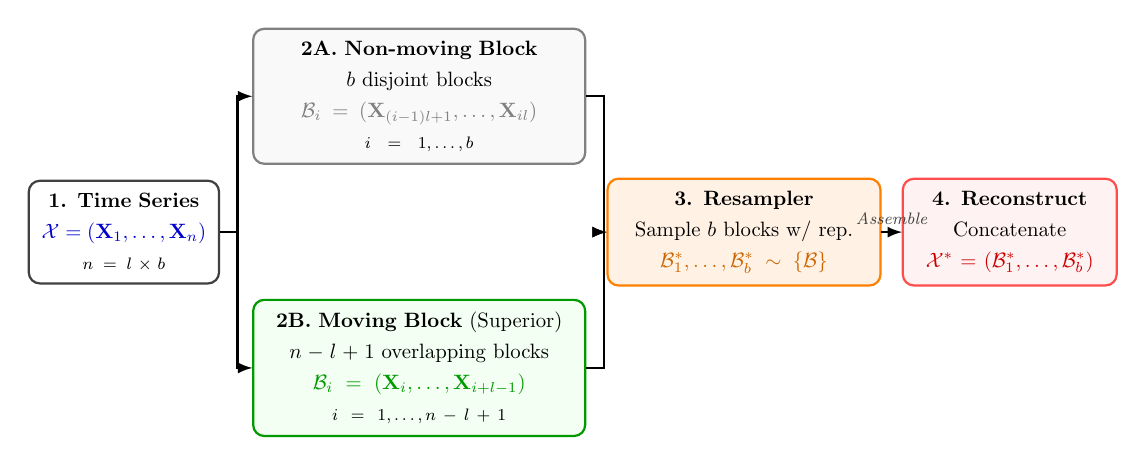
\begin{tikzpicture}[
        scale=0.75, transform shape,
        ->, >=latex, thick,
        basebox/.style={draw=darkgray, thick, rounded corners, fill=white, align=center, inner sep=6pt},
        note/.style={font=\footnotesize\itshape, text=darkgray}
    ]

        % 1. Input Data (Đẩy vào gốc tọa độ, thu hẹp width)
        \node[basebox, text width=2.8cm] (data) at (0, 0) {
            \textbf{1. Time Series} \\ \vspace{0.1cm}
            {\color{blue!80!black}\textbf{$\mathcal{X} = (\mathbf{X}_1, \dots, \mathbf{X}_n)$}} \\ \vspace{0.1cm}
            \footnotesize $n = l \times b$
        };

        % 2. Partitioning Strategies (Kéo tọa độ X từ 6 về 5)
        \node[basebox, text width=5.2cm, draw=gray, fill=gray!5] (nonmoving) at (5, 2.3) {
            \textbf{2A. Non-moving Block} \\ \vspace{0.1cm}
            $b$ disjoint blocks \\ \vspace{0.1cm}
            {\color{gray}\textbf{$\mathcal{B}_i = (\mathbf{X}_{(i-1)l+1}, \dots, \mathbf{X}_{il})$}} \\ \vspace{0.1cm}
            \footnotesize $i = 1, \dots, b$
        };

        \node[basebox, text width=5.2cm, draw=green!60!black, fill=green!5] (moving) at (5, -2.3) {
            \textbf{2B. Moving Block} (Superior) \\ \vspace{0.1cm}
            $n-l+1$ overlapping blocks \\ \vspace{0.1cm}
            {\color{green!60!black}\textbf{$\mathcal{B}_i = (\mathbf{X}_i, \dots, \mathbf{X}_{i+l-1})$}} \\ \vspace{0.1cm}
            \footnotesize $i = 1, \dots, n-l+1$
        };

        % 3. Resampling Engine (Kéo tọa độ X từ 12.5 về 10.5)
        \node[basebox, text width=4.2cm, draw=orange, fill=orange!10] (resample) at (10.5, 0) {
            \textbf{3. Resampler} \\ \vspace{0.1cm}
            Sample $b$ blocks w/ rep. \\ \vspace{0.1cm}
            {\color{orange!80!black}\textbf{$\mathcal{B}_1^*, \dots, \mathcal{B}_b^* \sim \{ \mathcal{B} \}$}}
        };

        % 4. Pseudo-dataset (Kéo tọa độ X từ 17.5 về 15)
        \node[basebox, text width=3.2cm, draw=red!70, fill=red!5] (pseudo) at (15, 0) {
            \textbf{4. Reconstruct} \\ \vspace{0.1cm}
            Concatenate \\ \vspace{0.1cm}
            {\color{red!80!black}\textbf{$\mathcal{X}^* = (\mathcal{B}_1^*, \dots, \mathcal{B}_b^*)$}}
        };

        % --- Vẽ đường nối (Chỉnh độ dài góc cua từ 0.5 xuống 0.3 cho gọn) ---
        \draw (data.east) -- ++(0.3,0) |- (nonmoving.west);
        \draw (data.east) -- ++(0.3,0) |- (moving.west);

        \draw (nonmoving.east) -- ++(0.3,0) |- (resample.west);
        \draw (moving.east) -- ++(0.3,0) |- (resample.west);

        \draw (resample.east) -- node[above, note] {Assemble} (pseudo.west);

    \end{tikzpicture}
    \end{center}
\end{frame}